\section{Improving Deep Neural Networks: Hyperparameter tuning, Regularization and Optimization}

\subsection{Practical aspects of Deep Learning}

Welcome to the first assignment of the hyper parameters tuning specialization. It is very important that you regularize your model properly because it could dramatically improve your results.
\begin{figure}[h]
\begin{center}
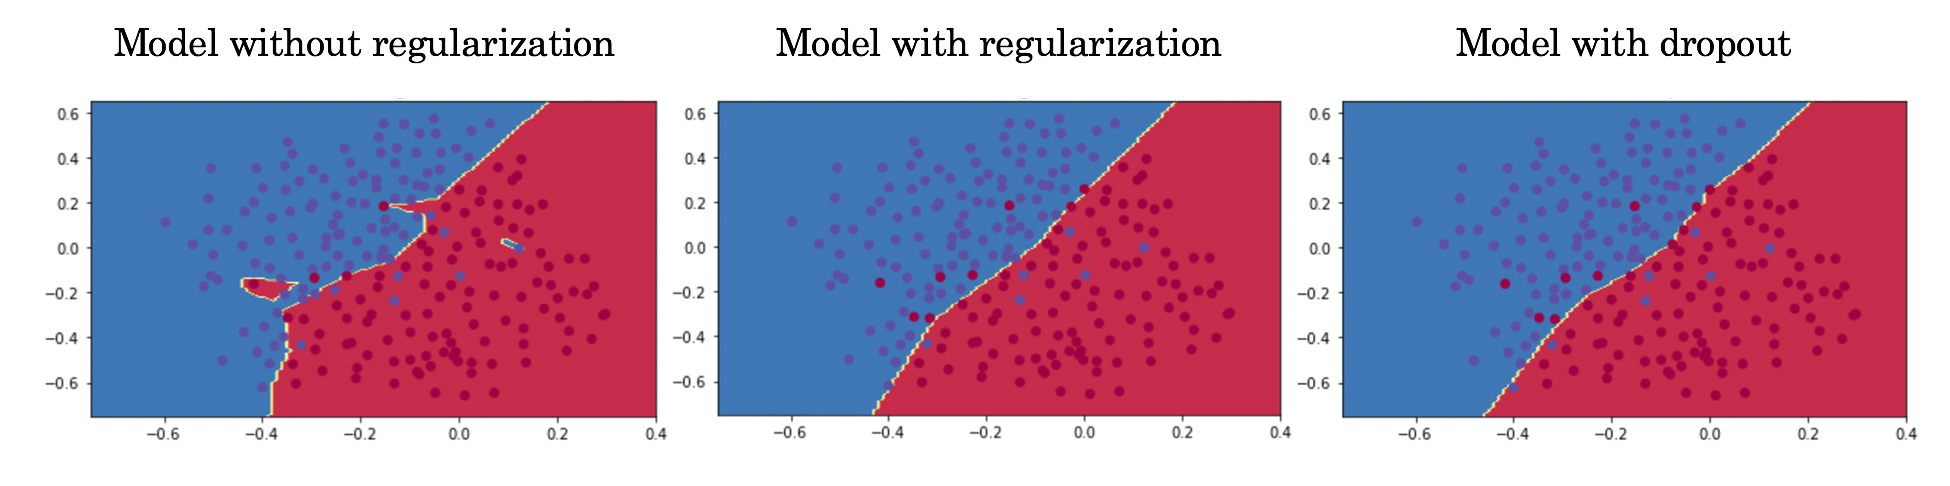
\includegraphics[width=\textwidth]{course2/Initialization}
\end{center}
\end{figure}

By completing this assignment you will:
\begin{itemize}
\item Understand that different regularization methods that could help your model.
\item Implement dropout and see it work on data.
\item Recognize that a model without regularization gives you a better accuracy on the training set but nor necessarily on the test set.
\item Understand that you could use both dropout and regularization on your model.
\end{itemize}

This assignment prepares you well for the upcoming assignment. Take your time to complete it and make sure you get the expected outputs when working through the different exercises. In some code blocks, you will find a "\#GRADED FUNCTION: functionName" comment. Please do not modify it. After you are done, submit your work and check your results. You need to score 80\% to pass. Good luck :) !


\subsubsection{Initialization}

Welcome to the first assignment of ``Improving Deep Neural Networks".

Training your neural network requires specifying an initial value of the weights. A well chosen initialization method will help learning.

If you completed the previous course of this specialization, you probably followed our instructions for weight initialization, and it has worked out so far. But how do you choose the initialization for a new neural network? In this notebook, you will see how different initializations lead to different results.

A well chosen initialization can:
\begin{itemize}
\item Speed up the convergence of gradient descent
\item Increase the odds of gradient descent converging to a lower training (and generalization) error
\end{itemize}


\subsubsubsection{Packages}
To get started, run the following code to load the packages and the planar dataset you will try to classify.
\begin{minted}{python}
import numpy as np
import matplotlib.pyplot as plt
import sklearn
import sklearn.datasets
from init_utils import sigmoid, relu, compute_loss, forward_propagation, backward_propagation
from init_utils import update_parameters, predict, load_dataset, plot_decision_boundary, predict_dec

# matplotlib inline
plt.rcParams['figure.figsize'] = (7.0, 4.0) # set default size of plots
plt.rcParams['image.interpolation'] = 'nearest'
plt.rcParams['image.cmap'] = 'gray'

# load image dataset: blue/red dots in circles
train_X, train_Y, test_X, test_Y = load_dataset()
\end{minted}
\begin{figure}[h]
\begin{center}
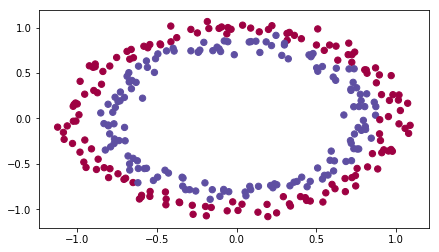
\includegraphics[width=0.7\textwidth]{course2/blue_red_dots}
\end{center}
\end{figure}

You would like a classifier to separate the blue dots from the red dots.


\subsubsubsection{Neural Network model}

You will use a 3-layer neural network (already implemented for you). Here are the initialization methods you will experiment with:
\begin{itemize}
\item \emph{Zeros initialization} -- setting initialization = ``zeros" in the input argument.
\item \emph{Random initialization} -- setting initialization = ``random" in the input argument. This initializes the weights to large random values.
\item \emph{He initialization} -- setting initialization = ``he" in the input argument. This initializes the weights to random values scaled according to a paper by \href{https://arxiv.org/abs/1512.03385}{He et al., 2015}.
\end{itemize}
{\textbf {Instructions}}: Please quickly read over the code below, and run it. In the next part you will implement the three initialization methods that this model() calls.

\begin{minted}{python}
def model(X, Y, learning_rate = 0.01, num_iterations = 15000, print_cost = True, initialization = "he"):
    """
    Implements a three-layer neural network: LINEAR->RELU->LINEAR->RELU->LINEAR->SIGMOID.
    
    Arguments:
    X -- input data, of shape (2, number of examples)
    Y -- true "label" vector (containing 0 for red dots; 1 for blue dots), of shape (1, number of examples)
    learning_rate -- learning rate for gradient descent 
    num_iterations -- number of iterations to run gradient descent
    print_cost -- if True, print the cost every 1000 iterations
    initialization -- flag to choose which initialization to use ("zeros","random" or "he")
    
    Returns:
    parameters -- parameters learnt by the model
    """
        
    grads = {}
    costs = [] # to keep track of the loss
    m = X.shape[1] # number of examples
    layers_dims = [X.shape[0], 10, 5, 1]
    
    # Initialize parameters dictionary.
    if initialization == "zeros":
        parameters = initialize_parameters_zeros(layers_dims)
    elif initialization == "random":
        parameters = initialize_parameters_random(layers_dims)
    elif initialization == "he":
        parameters = initialize_parameters_he(layers_dims)

    # Loop (gradient descent)

    for i in range(0, num_iterations):

        # Forward propagation: LINEAR -> RELU -> LINEAR -> RELU -> LINEAR -> SIGMOID.
        a3, cache = forward_propagation(X, parameters)
        
        # Loss
        cost = compute_loss(a3, Y)

        # Backward propagation.
        grads = backward_propagation(X, Y, cache)
        
        # Update parameters.
        parameters = update_parameters(parameters, grads, learning_rate)
        
        # Print the loss every 1000 iterations
        if print_cost and i % 1000 == 0:
            print("Cost after iteration {}: {}".format(i, cost))
            costs.append(cost)
            
    # plot the loss
    plt.plot(costs)
    plt.ylabel('cost')
    plt.xlabel('iterations (per hundreds)')
    plt.title("Learning rate =" + str(learning_rate))
    plt.show()
    
    return parameters
\end{minted}


\subsubsubsection{Zero initialization}

There are two types of parameters to initialize in a neural network:
\begin{itemize}
\item the weight matrices $(W^{[1]}, W^{[2]}, W^{[3]}, ..., W^{[L-1]}, W^{[L]})$
\item the bias vectors $(b^{[1]}, b^{[2]}, b^{[3]}, ..., b^{[L-1]}, b^{[L]})$
\end{itemize}

{\textbf {Exercise}}: Implement the following function to initialize all parameters to zeros. You'll see later that this does not work well since it fails to "break symmetry", but lets try it anyway and see what happens. Use np.zeros((..,..)) with the correct shapes.
\begin{minted}{python}
# GRADED FUNCTION: initialize_parameters_zeros 
def initialize_parameters_zeros(layers_dims):
    """
    Arguments:
    layer_dims -- python array (list) containing the size of each layer.
    
    Returns:
    parameters -- python dictionary containing your parameters "W1", "b1", ..., "WL", "bL":
            W1 -- weight matrix of shape (layers_dims[1], layers_dims[0])
            b1 -- bias vector of shape (layers_dims[1], 1)
                  ...
            WL -- weight matrix of shape (layers_dims[L], layers_dims[L-1])
            bL -- bias vector of shape (layers_dims[L], 1)
    """
    
    parameters = {}
    L = len(layers_dims)            # number of layers in the network
    
    for l in range(1, L):
        ### START CODE HERE ### (≈ 2 lines of code)
        parameters['W' + str(l)] = np.zeros((layers_dims[l],layers_dims[l-1])) 
        parameters['b' + str(l)] = np.zeros((layers_dims[l],1)) 
        ### END CODE HERE ###
    return parameters
\end{minted}

\begin{minted}{python}
parameters = initialize_parameters_zeros([3,2,1])
print("W1 = " + str(parameters["W1"]))
print("b1 = " + str(parameters["b1"]))
print("W2 = " + str(parameters["W2"]))
print("b2 = " + str(parameters["b2"]))

#output
W1 = [[ 0.  0.  0.]
 [ 0.  0.  0.]]
b1 = [[ 0.]
 [ 0.]]
W2 = [[ 0.  0.]]
b2 = [[ 0.]]

\end{minted}

Run the following code to train your model on 15,000 iterations using zeros initialization.
\begin{minted}{python}
parameters = model(train_X, train_Y, initialization = "zeros")
print ("On the train set:")
predictions_train = predict(train_X, train_Y, parameters)
print ("On the test set:")
predictions_test = predict(test_X, test_Y, parameters)
\end{minted}
\begin{minted}{python}
#output
Cost after iteration 0: 0.6931471805599453
Cost after iteration 1000: 0.6931471805599453
Cost after iteration 2000: 0.6931471805599453
Cost after iteration 3000: 0.6931471805599453
Cost after iteration 4000: 0.6931471805599453
Cost after iteration 5000: 0.6931471805599453
Cost after iteration 6000: 0.6931471805599453
Cost after iteration 7000: 0.6931471805599453
Cost after iteration 8000: 0.6931471805599453
Cost after iteration 9000: 0.6931471805599453
Cost after iteration 10000: 0.6931471805599455
Cost after iteration 11000: 0.6931471805599453
Cost after iteration 12000: 0.6931471805599453
Cost after iteration 13000: 0.6931471805599453
Cost after iteration 14000: 0.6931471805599453

On the train set:
Accuracy: 0.5
On the test set:
Accuracy: 0.5
\end{minted}

\begin{figure}[h]
\begin{center}
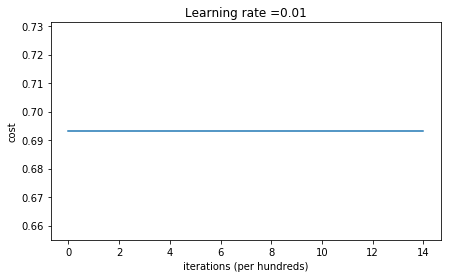
\includegraphics[width=0.7\textwidth]{course2/initialize_parameters_zeros_cost}
\end{center}
\end{figure}

The performance is really bad, and the cost does not really decrease, and the algorithm performs no better than random guessing. Why? Lets look at the details of the predictions and the decision boundary:
\begin{minted}{python}
print ("predictions_train = " + str(predictions_train))
print ("predictions_test = " + str(predictions_test))

#output
predictions_train = [[0 0 0 0 0 0 0 0 0 0 0 0 0 0 0 0 0 0 0 0 0 0 0 0 0 0 0 0 0 0 0 0 0 0 0 0 0
  0 0 0 0 0 0 0 0 0 0 0 0 0 0 0 0 0 0 0 0 0 0 0 0 0 0 0 0 0 0 0 0 0 0 0 0 0
  0 0 0 0 0 0 0 0 0 0 0 0 0 0 0 0 0 0 0 0 0 0 0 0 0 0 0 0 0 0 0 0 0 0 0 0 0
  0 0 0 0 0 0 0 0 0 0 0 0 0 0 0 0 0 0 0 0 0 0 0 0 0 0 0 0 0 0 0 0 0 0 0 0 0
  0 0 0 0 0 0 0 0 0 0 0 0 0 0 0 0 0 0 0 0 0 0 0 0 0 0 0 0 0 0 0 0 0 0 0 0 0
  0 0 0 0 0 0 0 0 0 0 0 0 0 0 0 0 0 0 0 0 0 0 0 0 0 0 0 0 0 0 0 0 0 0 0 0 0
  0 0 0 0 0 0 0 0 0 0 0 0 0 0 0 0 0 0 0 0 0 0 0 0 0 0 0 0 0 0 0 0 0 0 0 0 0
  0 0 0 0 0 0 0 0 0 0 0 0 0 0 0 0 0 0 0 0 0 0 0 0 0 0 0 0 0 0 0 0 0 0 0 0 0
  0 0 0 0]]
predictions_test = [[0 0 0 0 0 0 0 0 0 0 0 0 0 0 0 0 0 0 0 0 0 0 0 0 0 0 0 0 0 0 0 0 0 0 0 0 0
  0 0 0 0 0 0 0 0 0 0 0 0 0 0 0 0 0 0 0 0 0 0 0 0 0 0 0 0 0 0 0 0 0 0 0 0 0
  0 0 0 0 0 0 0 0 0 0 0 0 0 0 0 0 0 0 0 0 0 0 0 0 0 0]]
\end{minted}
\begin{minted}{python}
plt.title("Model with Zeros initialization")
axes = plt.gca()
axes.set_xlim([-1.5,1.5])
axes.set_ylim([-1.5,1.5])
plot_decision_boundary(lambda x: predict_dec(parameters, x.T), train_X, train_Y)
\end{minted}
\begin{figure}[h]
\begin{center}
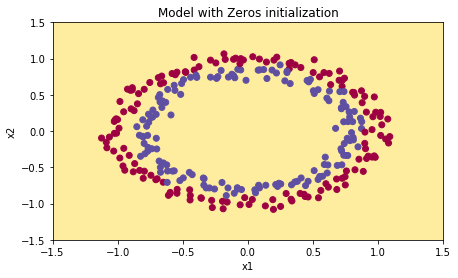
\includegraphics[width=0.7\textwidth]{course2/Model_with_Zeros_initialization}
\caption{Model with Zeros initialization}
\end{center}
\end{figure}

The model is predicting 0 for every example.

In general, initializing all the weights to zero results in the network failing to break symmetry. This means that every neuron in each layer will learn the same thing, and you might as well be training a neural network with  $n^{[l]}=1$  for every layer, and the network is no more powerful than a linear classifier such as logistic regression.

{\color{red} \textbf {
What you should remember:
\begin{itemize}
\item The weights  $W^{[l]}$  should be initialized randomly to break symmetry.
\item It is however okay to initialize the biases  $b^{[l]}$  to zeros. Symmetry is still broken so long as  $W^{[l]}$ is initialized randomly.
\end{itemize}
}}

\subsubsubsection{Random initialization}

To break symmetry, lets intialize the weights randomly. Following random initialization, each neuron can then proceed to learn a different function of its inputs. In this exercise, you will see what happens if the weights are intialized randomly, but to very large values.

{\textbf {Exercise}}: Implement the following function to initialize your weights to large random values (scaled by *10) and your biases to zeros. Use np.random.randn(..,..)*10 for weights and np.zeros((.., ..)) for biases. We are using a fixed np.random.seed(..) to make sure your ``random" weights match ours, so don't worry if running several times your code gives you always the same initial values for the parameters.

\begin{minted}{python}
# GRADED FUNCTION: initialize_parameters_random
def initialize_parameters_random(layers_dims):
    """
    Arguments:
    layer_dims -- python array (list) containing the size of each layer.
    
    Returns:
    parameters -- python dictionary containing your parameters "W1", "b1", ..., "WL", "bL":
                    W1 -- weight matrix of shape (layers_dims[1], layers_dims[0])
                    b1 -- bias vector of shape (layers_dims[1], 1)
                    ...
                    WL -- weight matrix of shape (layers_dims[L], layers_dims[L-1])
                    bL -- bias vector of shape (layers_dims[L], 1)
    """
    
    np.random.seed(3)               # This seed makes sure your "random" numbers will be the as ours
    parameters = {}
    L = len(layers_dims)            # integer representing the number of layers
    
    for l in range(1, L):
        ### START CODE HERE ### (≈ 2 lines of code)
        parameters['W' + str(l)] = np.random.randn(layers_dims[L], layers_dims[L-1]) * 10
        parameters['b' + str(l)] = np.zeros((layers_dims[L], 1))
        ### END CODE HERE ###

    return parameters
\end{minted}
\begin{minted}{python}
parameters = initialize_parameters_random([3, 2, 1])
print("W1 = " + str(parameters["W1"]))
print("b1 = " + str(parameters["b1"]))
print("W2 = " + str(parameters["W2"]))
print("b2 = " + str(parameters["b2"]))    

#output
W1 = [[ 17.88628473   4.36509851   0.96497468]
 [-18.63492703  -2.77388203  -3.54758979]]
b1 = [[ 0.]
 [ 0.]]
W2 = [[-0.82741481 -6.27000677]]
b2 = [[ 0.]]
\end{minted}

Run the following code to train your model on 15,000 iterations using random initialization.
\begin{minted}{python}
parameters = model(train_X, train_Y, initialization = "random")
print ("On the train set:")
predictions_train = predict(train_X, train_Y, parameters)
print ("On the test set:")
predictions_test = predict(test_X, test_Y, parameters)

#output
Cost after iteration 0: inf
Cost after iteration 1000: 0.6237287551108738
Cost after iteration 2000: 0.5981106708339466
......
Cost after iteration 14000: 0.38278397192120406

#Accuracy
On the train set:
Accuracy: 0.83
On the test set:
Accuracy: 0.86
\end{minted}
\vspace{-0.5cm}
\begin{figure}[h]
\begin{center}
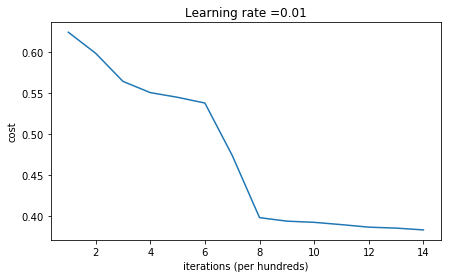
\includegraphics[width=0.7\textwidth]{course2/initialize_parameters_random_cost}
\end{center}
\end{figure}


If you see ``inf" as the cost after the iteration 0, this is because of numerical roundoff; a more numerically sophisticated implementation would fix this. But this isn't worth worrying about for our purposes.

Anyway, it looks like you have broken symmetry, and this gives better results. than before. The model is no longer outputting all 0s.

\begin{minted}{python}
print (predictions_train)
print (predictions_test)

#output
[[1 0 1 1 0 0 1 1 1 1 1 0 1 0 0 1 0 1 1 0 0 0 1 0 1 1 1 1 1 1 0 1 1 0 0 1 1
  1 1 1 1 1 1 0 1 1 1 1 0 1 0 1 1 1 1 0 0 1 1 1 1 0 1 1 0 1 0 1 1 1 1 0 0 0
  0 0 1 0 1 0 1 1 1 0 0 1 1 1 1 1 1 0 0 1 1 1 0 1 1 0 1 0 1 1 0 1 1 0 1 0 1
  1 0 0 1 0 0 1 1 0 1 1 1 0 1 0 0 1 0 1 1 1 1 1 1 1 0 1 1 0 0 1 1 0 0 0 1 0
  1 0 1 0 1 1 1 0 0 1 1 1 1 0 1 1 0 1 0 1 1 0 1 0 1 1 1 1 0 1 1 1 1 0 1 0 1
  0 1 1 1 1 0 1 1 0 1 1 0 1 1 0 1 0 1 1 1 0 1 1 1 0 1 0 1 0 0 1 0 1 1 0 1 1
  0 1 1 0 1 1 1 0 1 1 1 1 0 1 0 0 1 1 0 1 1 1 0 0 0 1 1 0 1 1 1 1 0 1 1 0 1
  1 1 0 0 1 0 0 0 1 0 0 0 1 1 1 1 0 0 0 0 1 1 1 1 0 0 1 1 1 1 1 1 1 0 0 0 1
  1 1 1 0]]
[[1 1 1 1 0 1 0 1 1 0 1 1 1 0 0 0 0 1 0 1 0 0 1 0 1 0 1 1 1 1 1 0 0 0 0 1 0
  1 1 0 0 1 1 1 1 1 0 1 1 1 0 1 0 1 1 0 1 0 1 0 1 1 1 1 1 1 1 1 1 0 1 0 1 1
  1 1 1 0 1 0 0 1 0 0 0 1 1 0 1 1 0 0 0 1 1 0 1 1 0 0]]
\end{minted}

\begin{figure}[h]
\begin{center}
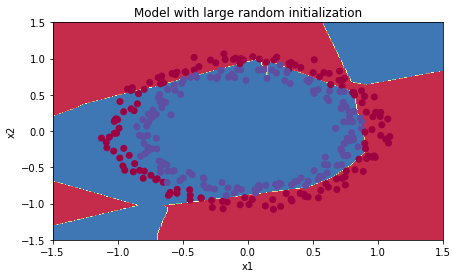
\includegraphics[width=0.6\textwidth]{course2/initialize_parameters_random}
\caption{Model with random initialization}
\end{center}
\end{figure}


\begin{minted}{python}
plt.title("Model with large random initialization")
axes = plt.gca()
axes.set_xlim([-1.5,1.5])
axes.set_ylim([-1.5,1.5])
plot_decision_boundary(lambda x: predict_dec(parameters, x.T), train_X, train_Y)
\end{minted}


{\textbf {Observations}}:
\begin{itemize}
\item The cost starts very high. This is because with large random-valued weights, the last activation (sigmoid) outputs results that are very close to 0 or 1 for some examples, and when it gets that example wrong it incurs a very high loss for that example. Indeed, when  $log(a^{[3]})=log(0)$, the loss goes to infinity.
\item Poor initialization can lead to vanishing/exploding gradients, which also slows down the optimization algorithm.
\item If you train this network longer you will see better results, but initializing with overly large random numbers slows down the optimization.
\end{itemize}

{\color{red} \textbf {In summary:
\begin{itemize}
\item Initializing weights to very large random values does not work well.
\item Hopefully intializing with small random values does better. The important question is: how small should be these random values be? Lets find out in the next part!
\end{itemize}
}}


\subsubsubsection{He initialization}

Finally, try ``He Initialization"; this is named for the first author of He et al., 2015. (If you have heard of ``Xavier initialization", this is similar except Xavier initialization uses a scaling factor for the weights $W^{[l]}$ of \emph{sqrt(1./layers\_dims[l-1])} where He initialization would use \emph{sqrt(2./layers\_dims[l-1])}.)

{\textbf {Exercise}}: Implement the following function to initialize your parameters with He initialization.

{\textbf {Hint}}: This function is similar to the previous \emph{initialize\_parameters\_random(...)}. The only difference is that instead of multiplying \emph{np.random.randn(..,..)} by 10, you will multiply it by $\sqrt{\frac{2}{\text{dimension of the previous layer}}}$, which is what He initialization recommends for layers with a ReLU activation. 

\begin{minted}{python}
# GRADED FUNCTION: initialize_parameters_he
def initialize_parameters_he(layers_dims):
    """
    Arguments:
    layer_dims -- python array (list) containing the size of each layer.
    
    Returns:
    parameters -- python dictionary containing your parameters "W1", "b1", ..., "WL", "bL":
                    W1 -- weight matrix of shape (layers_dims[1], layers_dims[0])
                    b1 -- bias vector of shape (layers_dims[1], 1)
                    ...
                    WL -- weight matrix of shape (layers_dims[L], layers_dims[L-1])
                    bL -- bias vector of shape (layers_dims[L], 1)
    """
    
    np.random.seed(3)
    parameters = {}
    L = len(layers_dims) - 1 # integer representing the number of layers
     
    for l in range(1, L + 1):
        ### START CODE HERE ### (≈ 2 lines of code)
        parameters['W' + str(l)] = np.random.randn(layers_dims[l], layers_dims[l-1]) * np.sqrt(2./layers_dims[l-1])
        parameters['b' + str(l)] = np.zeros((layers_dims[l], 1))
        ### END CODE HERE ###
        
    return parameters
\end{minted}

\begin{minted}{python}
parameters = initialize_parameters_he([2, 4, 1])
print("W1 = " + str(parameters["W1"]))
print("b1 = " + str(parameters["b1"]))
print("W2 = " + str(parameters["W2"]))
print("b2 = " + str(parameters["b2"]))

#output
1 = [[ 1.78862847  0.43650985]
 [ 0.09649747 -1.8634927 ]
 [-0.2773882  -0.35475898]
 [-0.08274148 -0.62700068]]
b1 = [[ 0.]
 [ 0.]
 [ 0.]
 [ 0.]]
W2 = [[-0.03098412 -0.33744411 -0.92904268  0.62552248]]
b2 = [[ 0.]]
\end{minted}

Run the following code to train your model on 15,000 iterations using He initialization.
\vspace{-0.5cm}
\begin{minted}{python}
parameters = model(train_X, train_Y, initialization = "he")
print ("On the train set:")
predictions_train = predict(train_X, train_Y, parameters)
print ("On the test set:")
predictions_test = predict(test_X, test_Y, parameters)

#output
Cost after iteration 0: 0.8830537463419761
Cost after iteration 1000: 0.6879825919728063
......
Cost after iteration 13000: 0.0845705595402428
Cost after iteration 14000: 0.07357895962677366

#Accuracy
On the train set:
Accuracy: 0.993333333333
On the test set:
Accuracy: 0.96

\end{minted}

\vspace{-0.3cm}
\begin{figure}[h]
\begin{center}
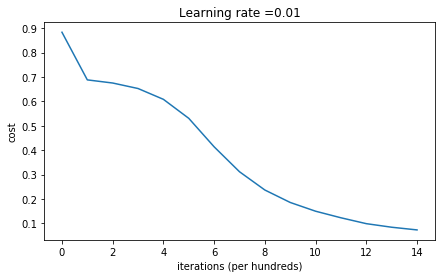
\includegraphics[width=0.6\textwidth]{course2/initialize_parameters_HE_cost}
\end{center}
\end{figure}

\vspace{-1cm}
\begin{minted}{python}
plt.title("Model with He initialization")
axes = plt.gca()
axes.set_xlim([-1.5,1.5])
axes.set_ylim([-1.5,1.5])
plot_decision_boundary(lambda x: predict_dec(parameters, x.T), train_X, train_Y)
\end{minted}

\begin{figure}[h]
\begin{center}
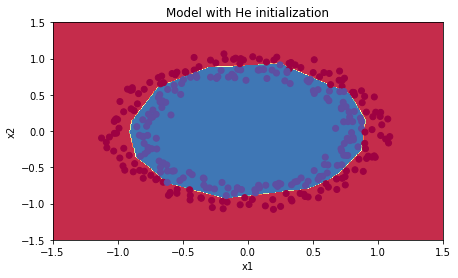
\includegraphics[width=0.6\textwidth]{course2/initialize_parameters_HE}
\caption{Model with He initialization}
\end{center}
\end{figure}


{\textbf {Observations}}:

The model with He initialization separates the blue and the red dots very well in a small number of iterations.


\subsubsubsection{Conclusions}

You have seen three different types of initializations. For the same number of iterations and same hyperparameters the comparison is:
\begin{table}[H]
\centering
\begin{tabular}{ccc}  
\toprule
Model&	Train accuracy	&Problem/Comment\\
\midrule
3-layer NN with zeros initialization	& 50\%	& fails to break symmetry\\
3-layer NN with large random initialization	& 83\%	& too large weights\\
3-layer NN with He initialization	&99\%	& recommended method\\
\bottomrule
\end{tabular}
\end{table}

{\color{red} \textbf{
What you should remember from this assignment:
\begin{itemize}
\item Different initializations lead to different results
\item Random initialization is used to break symmetry and make sure different hidden units can learn different things
\item Don't intialize to values that are too large
\item He initialization works well for networks with ReLU activations.
\end{itemize}
}}



\clearpage
\subsubsubsection{Code of initialization}
\begin{minted}{python}
import numpy as np
import matplotlib.pyplot as plt
import sklearn
import sklearn.datasets
from init_utils import sigmoid, relu, compute_loss, forward_propagation, backward_propagation
from init_utils import update_parameters, predict, load_dataset, plot_decision_boundary, predict_dec

#===========================================
# # matplotlib inline
# plt.rcParams['figure.figsize'] = (7.0, 4.0) # set default size of plots
# plt.rcParams['image.interpolation'] = 'nearest'
# plt.rcParams['image.cmap'] = 'gray'
#===========================================

# load image dataset: blue/red dots in circles
#train_X, train_Y, test_X, test_Y = load_dataset()

def model(X, Y, learning_rate = 0.01, num_iterations = 15000, print_cost = True, initialization = "he"):
    """
    Implements a three-layer neural network: LINEAR->RELU->LINEAR->RELU->LINEAR->SIGMOID.
    
    Arguments:
    X -- input data, of shape (2, number of examples)
    Y -- true "label" vector (containing 0 for red dots; 1 for blue dots), of shape (1, number of examples)
    learning_rate -- learning rate for gradient descent 
    num_iterations -- number of iterations to run gradient descent
    print_cost -- if True, print the cost every 1000 iterations
    initialization -- flag to choose which initialization to use ("zeros","random" or "he")
    
    Returns:
    parameters -- parameters learnt by the model
    """
        
    grads = {}
    costs = [] # to keep track of the loss
    m = X.shape[1] # number of examples
    layers_dims = [X.shape[0], 10, 5, 1]
    
    # Initialize parameters dictionary.
    if initialization == "zeros":
        parameters = initialize_parameters_zeros(layers_dims)
    elif initialization == "random":
        parameters = initialize_parameters_random(layers_dims)
    elif initialization == "he":
        parameters = initialize_parameters_he(layers_dims)

    # Loop (gradient descent)
    for i in range(0, num_iterations):

        # Forward propagation: LINEAR -> RELU -> LINEAR -> RELU -> LINEAR -> SIGMOID.
        a3, cache = forward_propagation(X, parameters)
        
        # Loss
        cost = compute_loss(a3, Y)

        # Backward propagation.
        grads = backward_propagation(X, Y, cache)
        
        # Update parameters.
        parameters = update_parameters(parameters, grads, learning_rate)
        
        # Print the loss every 1000 iterations
        if print_cost and i % 1000 == 0:
            print("Cost after iteration {}: {}".format(i, cost))
            costs.append(cost)
            
    # plot the loss
    plt.plot(costs)
    plt.ylabel('cost')
    plt.xlabel('iterations (per hundreds)')
    plt.title("Learning rate =" + str(learning_rate))
    plt.show()
    
    return parameters


# GRADED FUNCTION: initialize_parameters_zeros 
def initialize_parameters_zeros(layers_dims):
    """
    Arguments:
    layer_dims -- python array (list) containing the size of each layer.
    
    Returns:
    parameters -- python dictionary containing your parameters "W1", "b1", ..., "WL", "bL":
                    W1 -- weight matrix of shape (layers_dims[1], layers_dims[0])
                    b1 -- bias vector of shape (layers_dims[1], 1)
                    ...
                    WL -- weight matrix of shape (layers_dims[L], layers_dims[L-1])
                    bL -- bias vector of shape (layers_dims[L], 1)
    """
    
    parameters = {}
    L = len(layers_dims)            # number of layers in the network
    
    for l in range(1, L):
        parameters['W' + str(l)] = np.zeros((layers_dims[l],layers_dims[l-1])) 
        parameters['b' + str(l)] = np.zeros((layers_dims[l],1)) 
    return parameters


# GRADED FUNCTION: initialize_parameters_random
def initialize_parameters_random(layers_dims):
    """
    Arguments:
    layer_dims -- python array (list) containing the size of each layer.
    
    Returns:
    parameters -- python dictionary containing your parameters "W1", "b1", ..., "WL", "bL":
                    W1 -- weight matrix of shape (layers_dims[1], layers_dims[0])
                    b1 -- bias vector of shape (layers_dims[1], 1)
                    ...
                    WL -- weight matrix of shape (layers_dims[L], layers_dims[L-1])
                    bL -- bias vector of shape (layers_dims[L], 1)
    """
    
    np.random.seed(3)  # This seed makes sure your "random" numbers will be the as ours
    parameters = {}
    L = len(layers_dims)  # integer representing the number of layers
    
    for l in range(1, L):
        parameters['W' + str(l)] = np.random.randn(layers_dims[l], layers_dims[l-1]) * 10
        parameters['b' + str(l)] = np.zeros((layers_dims[l], 1))

    return parameters


# GRADED FUNCTION: initialize_parameters_he
def initialize_parameters_he(layers_dims):
    """
    Arguments:
    layer_dims -- python array (list) containing the size of each layer.
    
    Returns:
    parameters -- python dictionary containing your parameters "W1", "b1", ..., "WL", "bL":
                    W1 -- weight matrix of shape (layers_dims[1], layers_dims[0])
                    b1 -- bias vector of shape (layers_dims[1], 1)
                    ...
                    WL -- weight matrix of shape (layers_dims[L], layers_dims[L-1])
                    bL -- bias vector of shape (layers_dims[L], 1)
    """
    
    np.random.seed(3)
    parameters = {}
    L = len(layers_dims) - 1 # integer representing the number of layers
     
    for l in range(1, L + 1):
        parameters['W' + str(l)] = np.random.randn(layers_dims[l], layers_dims[l-1]) * np.sqrt(2./layers_dims[l-1])
        parameters['b' + str(l)] = np.zeros((layers_dims[l], 1))
        
    return parameters


#parameters = initialize_parameters_zeros([3,2,1])
#parameters = initialize_parameters_random([3, 2, 1])
parameters = initialize_parameters_he([2, 4, 1])
print("W1 = " + str(parameters["W1"]))
print("b1 = " + str(parameters["b1"]))
print("W2 = " + str(parameters["W2"]))
print("b2 = " + str(parameters["b2"]))

parameters = model(train_X, train_Y, initialization = "he")
print ("On the train set:")
predictions_train = predict(train_X, train_Y, parameters)
print ("On the test set:")
predictions_test = predict(test_X, test_Y, parameters)

plt.title("Model with He initialization")
axes = plt.gca()
axes.set_xlim([-1.5,1.5])
axes.set_ylim([-1.5,1.5])
plot_decision_boundary(lambda x: predict_dec(parameters, x.T), train_X, train_Y)
\end{minted}
\clearpage